\section{MODELING}
\label{sec:modeling}
In this section, we describe the dynamic model and control of a basic flapping-wing drone.
\begin{figure}[t]
    \centering
    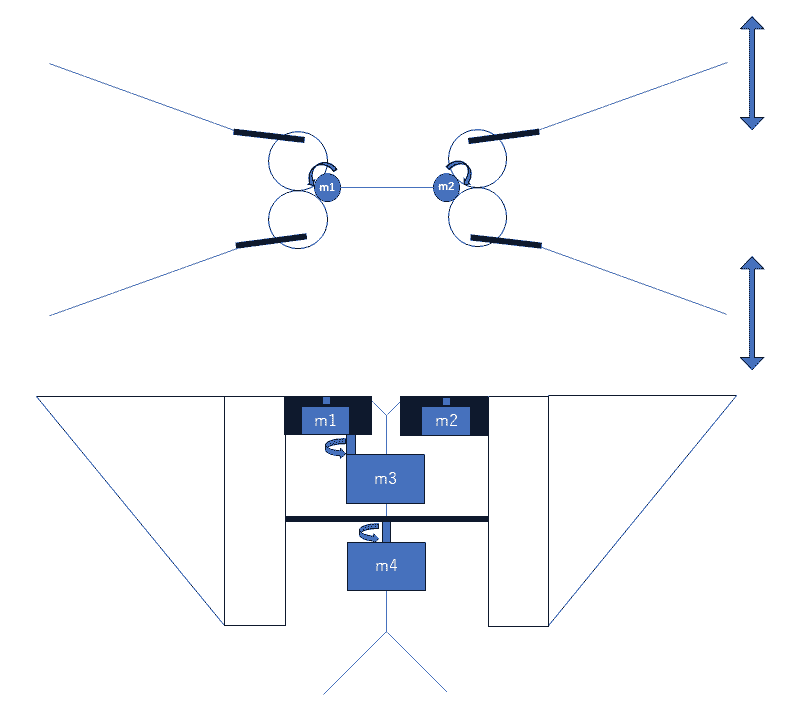
\includegraphics[width=\columnwidth]{modeling.png}
    \caption{The mechanical structure model of a tailless aerial robotic flapper. It has motors for thrust (m1, m2), a motor for pitch control (m3), and a motor for yaw control (m4).}
    \label{figure:modeling}
  \end{figure}
There are various types of flapping-wing drones, and we focus on a tailless aerial robotic flapper model~\cite{karasek2018tailless}, as shown in Fig.~\ref{figure:modeling}.
The drone is mounted with four motors: two motors for thrust (m1, m2), one motor for pitch control (m3), and one motor for yaw control (m4).
We can treat the dynamics as a single rigid body as follows:
\begin{equation}
    \begin{aligned}
      &m\bm{a} = m\bm{g} + \it{R}\bm{f}\\
      &I\dot{\bm{\omega}} + \bm{\omega} \times I\bm{\omega} = \bm{\tau}
    \end{aligned}
\end{equation}
where $m$ is the mass of the drone, 
$\bm{a}$ is the acceleration of the drone,
$\bm{g}$ is the gravity vector,
$\it{R}$ is the rotation matrix of the drone,
$\bm{f}$ is the thrust force of the drone,
$I$ is the inertia matrix of the drone, 
\bm{$\omega$} is the angular velocity of the drone, 
and \bm{$\tau$} is the torque applied to the drone.
The thrust force $\bm{f}$ and the torque $\bm{\tau}$ can be represented as follows:
\begin{equation}
  \label{eq:control}
  \begin{aligned}
    \begin{bmatrix}
      \bm{f}\\
      \bm{\tau}
    \end{bmatrix}
    &=
    g(m_1\omega_1, m_2\omega_2, m_3\theta_3, m_4\theta_4)\\
  \end{aligned}
\end{equation}
where $\omega_i$ is the angular velocity of the motor $i$, $m_i$ is the coefficient of the motor $i$, $\theta_i$ is the angle of the motor $i$, and $g$ is the mapping function from $\mathbb{R}^4$ to $\mathbb{R}^6$.
Based on these equations, we can derive the following PID control law:
\begin{equation}
  \begin{aligned}
    &\bm{f}_d = {PID}_r(\bm{e}_r)
    &\bm{\tau}_d &= {PID}_R(\bm{e_\theta})\\
    &\bm{e_r} = \bm{r} - \bm{r}_d
    &\bm{e_\theta} &= \bm{\theta} - \bm{\theta}_d\\
  \end{aligned}
\end{equation}
where $\bm{f}_d$ is the desired thrust force, 
$\bm{\tau}_d$ is the desired torque, 
$PID_r$ is the PID controller for the position, 
$PID_R$ is the PID controller for the orientation, 
$\bm{e_r}$ is the error of the position, 
$\bm{e_\theta}$ is the error of the orientation, 
$\bm{\theta}$ is the orientation of the drone, 
and $\bm{\theta}_d$ is the desired orientation of the drone.
Then, we can calculate the desired motor inputs from the desired thrust force and torque using the mapping function $g$ in (\ref{eq:control}).